\documentclass[]{article}
\usepackage{lmodern}
\usepackage{amssymb,amsmath}
\usepackage{ifxetex,ifluatex}
\usepackage{fixltx2e} % provides \textsubscript
\ifnum 0\ifxetex 1\fi\ifluatex 1\fi=0 % if pdftex
  \usepackage[T1]{fontenc}
  \usepackage[utf8]{inputenc}
\else % if luatex or xelatex
  \ifxetex
    \usepackage{mathspec}
  \else
    \usepackage{fontspec}
  \fi
  \defaultfontfeatures{Ligatures=TeX,Scale=MatchLowercase}
\fi
% use upquote if available, for straight quotes in verbatim environments
\IfFileExists{upquote.sty}{\usepackage{upquote}}{}
% use microtype if available
\IfFileExists{microtype.sty}{%
\usepackage{microtype}
\UseMicrotypeSet[protrusion]{basicmath} % disable protrusion for tt fonts
}{}
\usepackage[margin=1in]{geometry}
\usepackage{hyperref}
\hypersetup{unicode=true,
            pdftitle={Assignment 1},
            pdfauthor={Group 11},
            pdfborder={0 0 0},
            breaklinks=true}
\urlstyle{same}  % don't use monospace font for urls
\usepackage{color}
\usepackage{fancyvrb}
\newcommand{\VerbBar}{|}
\newcommand{\VERB}{\Verb[commandchars=\\\{\}]}
\DefineVerbatimEnvironment{Highlighting}{Verbatim}{commandchars=\\\{\}}
% Add ',fontsize=\small' for more characters per line
\usepackage{framed}
\definecolor{shadecolor}{RGB}{248,248,248}
\newenvironment{Shaded}{\begin{snugshade}}{\end{snugshade}}
\newcommand{\KeywordTok}[1]{\textcolor[rgb]{0.13,0.29,0.53}{\textbf{#1}}}
\newcommand{\DataTypeTok}[1]{\textcolor[rgb]{0.13,0.29,0.53}{#1}}
\newcommand{\DecValTok}[1]{\textcolor[rgb]{0.00,0.00,0.81}{#1}}
\newcommand{\BaseNTok}[1]{\textcolor[rgb]{0.00,0.00,0.81}{#1}}
\newcommand{\FloatTok}[1]{\textcolor[rgb]{0.00,0.00,0.81}{#1}}
\newcommand{\ConstantTok}[1]{\textcolor[rgb]{0.00,0.00,0.00}{#1}}
\newcommand{\CharTok}[1]{\textcolor[rgb]{0.31,0.60,0.02}{#1}}
\newcommand{\SpecialCharTok}[1]{\textcolor[rgb]{0.00,0.00,0.00}{#1}}
\newcommand{\StringTok}[1]{\textcolor[rgb]{0.31,0.60,0.02}{#1}}
\newcommand{\VerbatimStringTok}[1]{\textcolor[rgb]{0.31,0.60,0.02}{#1}}
\newcommand{\SpecialStringTok}[1]{\textcolor[rgb]{0.31,0.60,0.02}{#1}}
\newcommand{\ImportTok}[1]{#1}
\newcommand{\CommentTok}[1]{\textcolor[rgb]{0.56,0.35,0.01}{\textit{#1}}}
\newcommand{\DocumentationTok}[1]{\textcolor[rgb]{0.56,0.35,0.01}{\textbf{\textit{#1}}}}
\newcommand{\AnnotationTok}[1]{\textcolor[rgb]{0.56,0.35,0.01}{\textbf{\textit{#1}}}}
\newcommand{\CommentVarTok}[1]{\textcolor[rgb]{0.56,0.35,0.01}{\textbf{\textit{#1}}}}
\newcommand{\OtherTok}[1]{\textcolor[rgb]{0.56,0.35,0.01}{#1}}
\newcommand{\FunctionTok}[1]{\textcolor[rgb]{0.00,0.00,0.00}{#1}}
\newcommand{\VariableTok}[1]{\textcolor[rgb]{0.00,0.00,0.00}{#1}}
\newcommand{\ControlFlowTok}[1]{\textcolor[rgb]{0.13,0.29,0.53}{\textbf{#1}}}
\newcommand{\OperatorTok}[1]{\textcolor[rgb]{0.81,0.36,0.00}{\textbf{#1}}}
\newcommand{\BuiltInTok}[1]{#1}
\newcommand{\ExtensionTok}[1]{#1}
\newcommand{\PreprocessorTok}[1]{\textcolor[rgb]{0.56,0.35,0.01}{\textit{#1}}}
\newcommand{\AttributeTok}[1]{\textcolor[rgb]{0.77,0.63,0.00}{#1}}
\newcommand{\RegionMarkerTok}[1]{#1}
\newcommand{\InformationTok}[1]{\textcolor[rgb]{0.56,0.35,0.01}{\textbf{\textit{#1}}}}
\newcommand{\WarningTok}[1]{\textcolor[rgb]{0.56,0.35,0.01}{\textbf{\textit{#1}}}}
\newcommand{\AlertTok}[1]{\textcolor[rgb]{0.94,0.16,0.16}{#1}}
\newcommand{\ErrorTok}[1]{\textcolor[rgb]{0.64,0.00,0.00}{\textbf{#1}}}
\newcommand{\NormalTok}[1]{#1}
\usepackage{graphicx,grffile}
\makeatletter
\def\maxwidth{\ifdim\Gin@nat@width>\linewidth\linewidth\else\Gin@nat@width\fi}
\def\maxheight{\ifdim\Gin@nat@height>\textheight\textheight\else\Gin@nat@height\fi}
\makeatother
% Scale images if necessary, so that they will not overflow the page
% margins by default, and it is still possible to overwrite the defaults
% using explicit options in \includegraphics[width, height, ...]{}
\setkeys{Gin}{width=\maxwidth,height=\maxheight,keepaspectratio}
\IfFileExists{parskip.sty}{%
\usepackage{parskip}
}{% else
\setlength{\parindent}{0pt}
\setlength{\parskip}{6pt plus 2pt minus 1pt}
}
\setlength{\emergencystretch}{3em}  % prevent overfull lines
\providecommand{\tightlist}{%
  \setlength{\itemsep}{0pt}\setlength{\parskip}{0pt}}
\setcounter{secnumdepth}{0}
% Redefines (sub)paragraphs to behave more like sections
\ifx\paragraph\undefined\else
\let\oldparagraph\paragraph
\renewcommand{\paragraph}[1]{\oldparagraph{#1}\mbox{}}
\fi
\ifx\subparagraph\undefined\else
\let\oldsubparagraph\subparagraph
\renewcommand{\subparagraph}[1]{\oldsubparagraph{#1}\mbox{}}
\fi

%%% Use protect on footnotes to avoid problems with footnotes in titles
\let\rmarkdownfootnote\footnote%
\def\footnote{\protect\rmarkdownfootnote}

%%% Change title format to be more compact
\usepackage{titling}

% Create subtitle command for use in maketitle
\newcommand{\subtitle}[1]{
  \posttitle{
    \begin{center}\large#1\end{center}
    }
}

\setlength{\droptitle}{-2em}
  \title{Assignment 1}
  \pretitle{\vspace{\droptitle}\centering\huge}
  \posttitle{\par}
  \author{Group 11}
  \preauthor{\centering\large\emph}
  \postauthor{\par}
  \predate{\centering\large\emph}
  \postdate{\par}
  \date{The Date}


\begin{document}
\maketitle

\section{0. Load Libraries and Dependencies}

\begin{Shaded}
\begin{Highlighting}[]
\KeywordTok{library}\NormalTok{(tidyverse)}
\KeywordTok{library}\NormalTok{(nFactors)}
\end{Highlighting}
\end{Shaded}

\section{1. Problem Statement}

The presented data from a conducted study shows the recovery status for
100 participants after taking two different drugs with differing doses.
Recovery is measured as the percentage drop in body pathogens before and
after taking the respective drug. In order to judge on the effectiveness
of the drugs the principal component analysis is applied, to shrink the
information to only a subset of the variables' dimensions. The
associated identification of useful factor brandings and the reflection
of the data on the identified subdimensions should help to evaluate the
initial question.\\
The second section starts with the data preparation and a brief
description of the data. Afterwards, in section three, the assumptions
for using principal component analysis are described including the way
we deal with them. In section four the principal component analysis is
applied and the most relevant outputs are described. The last section
covers the answering of first, how the factors in the subspace can be
labled appropriately and second, which drugs were effective.

\section{2. Descriptive Statistics}

Before dealing with the principal component analysis (PCA), it is
important to prepare the data. After importing the data and performing
the glimpse-function, one can see that the data is stored in a
data.frame object with the dimension 100x9.

\begin{Shaded}
\begin{Highlighting}[]
\NormalTok{drugdata <-}\StringTok{ }\KeywordTok{read.table}\NormalTok{(}\StringTok{"http://feb.kuleuven.be/martina.vandebroek/public/STATdata/drugsrecovery.txt"}\NormalTok{, }\DataTypeTok{header=}\NormalTok{T)}
\KeywordTok{class}\NormalTok{(drugdata)}
\end{Highlighting}
\end{Shaded}

\begin{verbatim}
## [1] "data.frame"
\end{verbatim}

\begin{Shaded}
\begin{Highlighting}[]
\KeywordTok{glimpse}\NormalTok{(drugdata)}
\end{Highlighting}
\end{Shaded}

\begin{verbatim}
## Observations: 100
## Variables: 9
## $ ID    <int> 1, 2, 3, 4, 5, 6, 7, 8, 9, 10, 11, 12, 13, 14, 15, 16, 1...
## $ L500  <int> 15, 10, 10, 10, 10, 20, 15, 5, 15, 10, 5, 20, 15, 20, 20...
## $ L1000 <int> 20, 15, 15, 15, 10, 20, 15, 5, 15, 10, 10, 20, 15, 30, 1...
## $ L2000 <int> 25, 5, 30, 5, 5, 20, 15, 5, 15, 5, 10, 25, 5, 20, 20, 20...
## $ L4000 <int> 30, 15, 30, 5, 25, 5, 35, 10, 55, 35, 20, 40, 30, 75, 30...
## $ R500  <int> 15, 15, 15, 5, 15, 15, 20, 5, 15, 5, 20, 10, 5, 20, 20, ...
## $ R1000 <int> 20, 20, 15, 10, 5, 20, 20, 10, 15, 10, 15, 10, 5, 20, 10...
## $ R2000 <int> 20, 20, 25, 5, 5, 15, 20, 15, 5, 5, 5, 20, 5, 15, 15, 20...
## $ R4000 <int> 30, 30, 40, 25, 65, 35, 25, 20, 25, 30, 20, 30, 25, 65, ...
\end{verbatim}

First of all the first column has to be eliminated, as it only stores
the ID values. It would be a major mistake taking this column into
account when performing PCA, as the results would be heavily biased.

\begin{Shaded}
\begin{Highlighting}[]
\NormalTok{drugdata <-}\StringTok{ }\NormalTok{drugdata[}\OperatorTok{-}\DecValTok{1}\NormalTok{]}
\KeywordTok{glimpse}\NormalTok{(drugdata)}
\end{Highlighting}
\end{Shaded}

\begin{verbatim}
## Observations: 100
## Variables: 8
## $ L500  <int> 15, 10, 10, 10, 10, 20, 15, 5, 15, 10, 5, 20, 15, 20, 20...
## $ L1000 <int> 20, 15, 15, 15, 10, 20, 15, 5, 15, 10, 10, 20, 15, 30, 1...
## $ L2000 <int> 25, 5, 30, 5, 5, 20, 15, 5, 15, 5, 10, 25, 5, 20, 20, 20...
## $ L4000 <int> 30, 15, 30, 5, 25, 5, 35, 10, 55, 35, 20, 40, 30, 75, 30...
## $ R500  <int> 15, 15, 15, 5, 15, 15, 20, 5, 15, 5, 20, 10, 5, 20, 20, ...
## $ R1000 <int> 20, 20, 15, 10, 5, 20, 20, 10, 15, 10, 15, 10, 5, 20, 10...
## $ R2000 <int> 20, 20, 25, 5, 5, 15, 20, 15, 5, 5, 5, 20, 5, 15, 15, 20...
## $ R4000 <int> 30, 30, 40, 25, 65, 35, 25, 20, 25, 30, 20, 30, 25, 65, ...
\end{verbatim}

One can also see that all the remaining values are of class integer.
This is important to know, as correlation matrices can only be
calculated using either integers or numerical values. After selecting
the relevant variables, it is also useful to check for missing values.
This is done by using the apply-function, which outputs the amount of
missing values for each column.

\begin{Shaded}
\begin{Highlighting}[]
\NormalTok{drugdata }\OperatorTok\StringTok{ }\KeywordTok{apply}\NormalTok{(}\DecValTok{2}\NormalTok{, }\ControlFlowTok{function}\NormalTok{(x)\{}
  \KeywordTok{sum}\NormalTok{(}\KeywordTok{is.na}\NormalTok{(x))}
\NormalTok{\}) }
\end{Highlighting}
\end{Shaded}

\begin{verbatim}
##  L500 L1000 L2000 L4000  R500 R1000 R2000 R4000 
##     0     0     0     0     0     0     0     0
\end{verbatim}

Hence, there arent any missing values presented in the data. Even though
the PCA has no distributional assumptions regarding the data it might
still be useful to get an idea of the distribution of the variables.

\begin{Shaded}
\begin{Highlighting}[]
\KeywordTok{summary}\NormalTok{(drugdata)}
\end{Highlighting}
\end{Shaded}

\begin{verbatim}
##       L500          L1000          L2000           L4000      
##  Min.   : 5.0   Min.   : 5.0   Min.   : 5.00   Min.   : 5.00  
##  1st Qu.: 5.0   1st Qu.:10.0   1st Qu.:10.00   1st Qu.:23.75  
##  Median :10.0   Median :15.0   Median :15.00   Median :35.00  
##  Mean   :12.2   Mean   :14.5   Mean   :17.00   Mean   :36.35  
##  3rd Qu.:20.0   3rd Qu.:20.0   3rd Qu.:21.25   3rd Qu.:50.00  
##  Max.   :30.0   Max.   :35.0   Max.   :60.00   Max.   :85.00  
##       R500          R1000          R2000          R4000      
##  Min.   : 5.0   Min.   : 5.0   Min.   : 5.0   Min.   : 5.00  
##  1st Qu.: 5.0   1st Qu.:10.0   1st Qu.:10.0   1st Qu.:20.00  
##  Median :10.0   Median :15.0   Median :15.0   Median :30.00  
##  Mean   :12.4   Mean   :14.3   Mean   :16.6   Mean   :36.35  
##  3rd Qu.:15.0   3rd Qu.:20.0   3rd Qu.:20.0   3rd Qu.:45.00  
##  Max.   :40.0   Max.   :35.0   Max.   :50.0   Max.   :90.00
\end{verbatim}

As one would expect, the range of the variables increase as the dose
increases. Taking into consideration that the minimum of each variable
is equal to five, this means that due to the higher dose there might be
at least some participants whose percentage drop in body pathogens was
quite high compared to the participants who got a lower dose. This can
also be derived when looking at the mean values or the outlier resistant
median values. This might give rise to the assumption that higher dose
is more effective. But let's see what is the outcome of the PCA.

\section{3. Assumptions}

When dealing with PCA there is basically one assumption which has to be
met, namely the variables have to be either mean centered or
standardized. As all variables are measured in the same scale (from 0\%
to 100\%) the variance observed to not artificial, but important
information which has to be considered. Therefore mean centering is
applied when perfoming PCA. This is done in the upcoming section when
using the prcomp-function with the center parameter set to TRUE.

\section{4. Method}

Before applying the method the first task is to identify the appropriate
number of principal components that effectively summarize the data.
Hence, we will decide based on two commonly used procedures. First by
visually analyzing the scree plot and second by performing Horn's
Parallel procedure.\\
The scree plot is just the visualization of the eigenvalues in
decreasing order. Hence, in the following chunk the eigenvalues are
extracted from the correlation matrix of the data and the eigenvalues
are ploted. The red line highlights the threshold value of one.

\begin{Shaded}
\begin{Highlighting}[]
\CommentTok{# Eigenvalues}
\NormalTok{eval <-}\StringTok{ }\KeywordTok{eigen}\NormalTok{(}\KeywordTok{cor}\NormalTok{(drugdata))}\OperatorTok{$}\NormalTok{values}

\CommentTok{# Scree Plot}
\KeywordTok{plot}\NormalTok{(eval, }\DataTypeTok{xlab =} \StringTok{"Principal Component"}\NormalTok{, }\DataTypeTok{ylab =} \StringTok{"Eigenvalue"}\NormalTok{,}
     \DataTypeTok{type =} \StringTok{"b"}\NormalTok{, }\DataTypeTok{main =} \StringTok{"Scree Plot"}\NormalTok{)}
\KeywordTok{abline}\NormalTok{(}\DataTypeTok{h=}\DecValTok{1}\NormalTok{,}\DataTypeTok{col=}\StringTok{"red"}\NormalTok{)}
\end{Highlighting}
\end{Shaded}

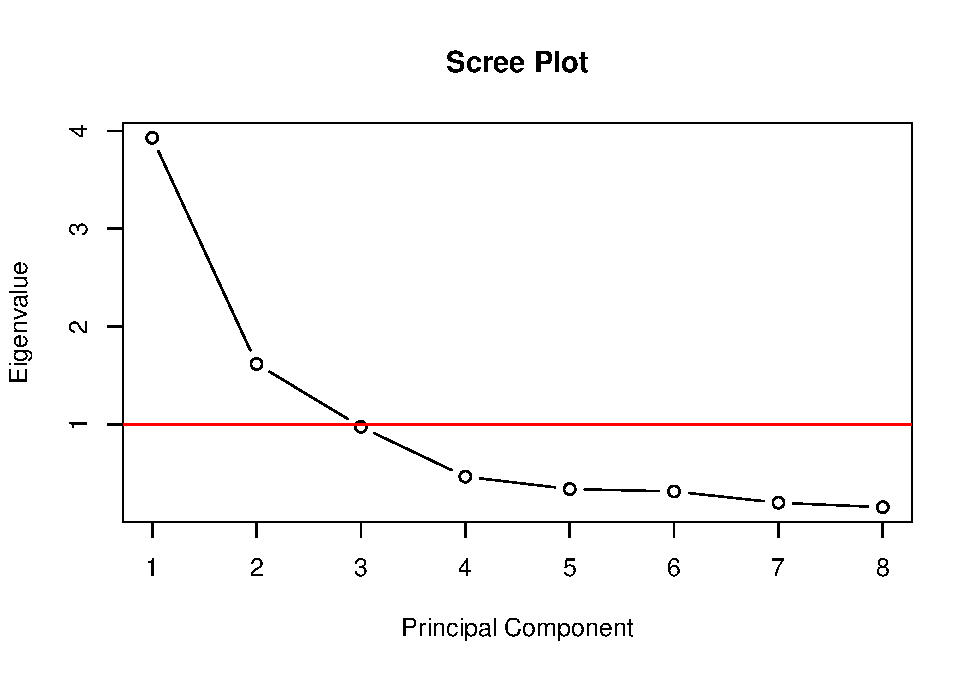
\includegraphics{assignment1_PCA_files/figure-latex/unnamed-chunk-6-1.pdf}

The first characteristic to find would be the so called elbow, which
separates the mountain from the debris. As the slope has almost an
exponential form, it is difficult to see whether such a distinction can
be made. The second criterion to check is to identify which eigenvalues
lay above the threshold value of one und which lay below. The first and
the second principal component are clearly above the threshold value.
The third principal component is a borderliner, as it's value of
0.9753248 lies slightly below the threshold value.

\begin{itemize}
\tightlist
\item
  Horn's Parallel procedure
\end{itemize}

Compute Eigenvalues associated with many simulated uncorrelated normal
variables - retain the ith PC if the corresponding eigenvalue is larger
than the 95th percentile of the distribution of the ith largest
eigenvalue of the random data (same idea as the previous rule but taking
random variation into account)

\begin{Shaded}
\begin{Highlighting}[]
\NormalTok{ap <-}\StringTok{ }\KeywordTok{parallel}\NormalTok{(}\DataTypeTok{subject =} \KeywordTok{nrow}\NormalTok{(drugdata), }\DataTypeTok{var =} \DecValTok{8}\NormalTok{, }\DataTypeTok{rep=} \DecValTok{1000}\NormalTok{,}\DataTypeTok{cent =} \FloatTok{0.05}\NormalTok{)}

\KeywordTok{plot}\NormalTok{(eval, }\DataTypeTok{xlim=}\KeywordTok{c}\NormalTok{(}\DecValTok{0}\NormalTok{,}\KeywordTok{ncol}\NormalTok{(drugdata)), }\DataTypeTok{ylim =} \KeywordTok{c}\NormalTok{(}\DecValTok{0}\NormalTok{,}\KeywordTok{max}\NormalTok{(eval)), }\DataTypeTok{ylab =} \StringTok{"eigenvalues"}\NormalTok{)}
\KeywordTok{lines}\NormalTok{(ap}\OperatorTok{$}\NormalTok{eigen}\OperatorTok{$}\NormalTok{qevpea, }\DataTypeTok{type =} \StringTok{"o"}\NormalTok{,}\DataTypeTok{pch =} \DecValTok{15}\NormalTok{, }\DataTypeTok{lwd =} \DecValTok{2}\NormalTok{,}\DataTypeTok{col =} \StringTok{"red"}\NormalTok{)}
\KeywordTok{title}\NormalTok{(}\DataTypeTok{main=} \StringTok{"Horn's parallel procedure - 5% lower percentile"}\NormalTok{)}
\end{Highlighting}
\end{Shaded}

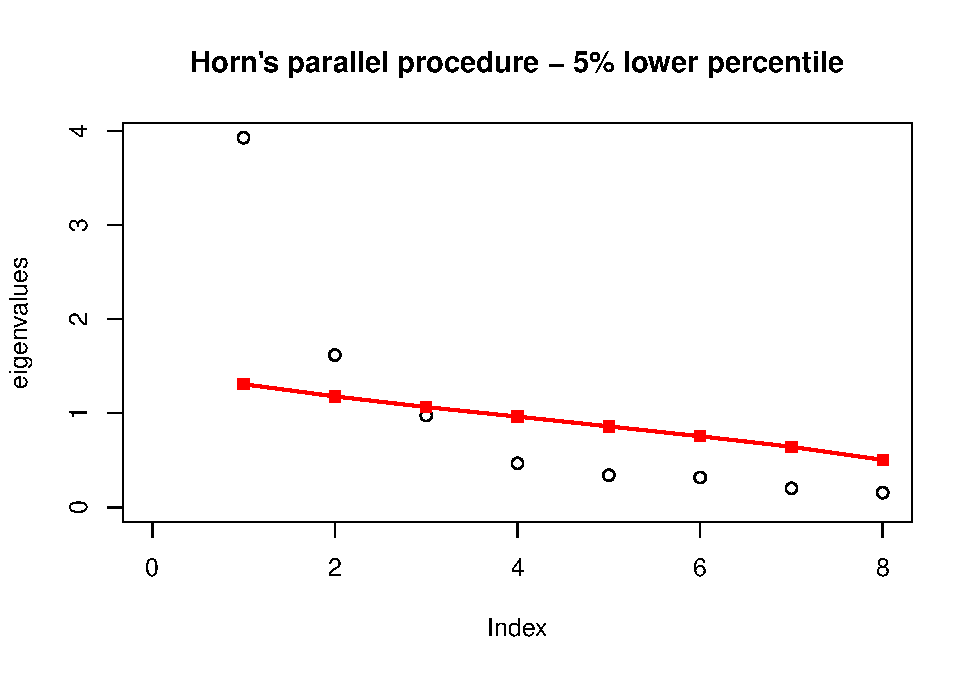
\includegraphics{assignment1_PCA_files/figure-latex/unnamed-chunk-7-1.pdf}

\begin{itemize}
\tightlist
\item
  Perform PCA
\end{itemize}

\begin{Shaded}
\begin{Highlighting}[]
\NormalTok{pr.out <-}\StringTok{ }\KeywordTok{prcomp}\NormalTok{(drugdata, }\DataTypeTok{center =} \OtherTok{TRUE}\NormalTok{)}
\end{Highlighting}
\end{Shaded}

\begin{itemize}
\tightlist
\item
  Variance explained
\end{itemize}

\begin{Shaded}
\begin{Highlighting}[]
\KeywordTok{summary}\NormalTok{(pr.out)}
\end{Highlighting}
\end{Shaded}

\begin{verbatim}
## Importance of components:
##                            PC1     PC2      PC3     PC4     PC5     PC6
## Standard deviation     26.5856 13.4059 10.55302 9.31934 5.41904 4.45328
## Proportion of Variance  0.6122  0.1557  0.09646 0.07523 0.02544 0.01718
## Cumulative Proportion   0.6122  0.7679  0.86434 0.93957 0.96500 0.98218
##                           PC7     PC8
## Standard deviation     3.6274 2.72292
## Proportion of Variance 0.0114 0.00642
## Cumulative Proportion  0.9936 1.00000
\end{verbatim}

\begin{Shaded}
\begin{Highlighting}[]
\CommentTok{# First two principal components explain 69.34% of the variance}

\CommentTok{# Variance Explained Plot}
\NormalTok{prop_varex <-}\StringTok{ }\NormalTok{eval }\OperatorTok{/}\StringTok{ }\KeywordTok{sum}\NormalTok{(eval)}
\KeywordTok{plot}\NormalTok{(prop_varex, }\DataTypeTok{xlab =} \StringTok{"Principal Component"}\NormalTok{, }\DataTypeTok{ylab =} \StringTok{"Proportion of varianve explained"}\NormalTok{,}
     \DataTypeTok{type =} \StringTok{"b"}\NormalTok{, }\DataTypeTok{main =} \StringTok{"Variance Explained"}\NormalTok{, }\DataTypeTok{ylim =} \KeywordTok{c}\NormalTok{(}\DecValTok{0}\NormalTok{,}\DecValTok{1}\NormalTok{))}
\KeywordTok{lines}\NormalTok{(}\KeywordTok{cumsum}\NormalTok{(prop_varex), }\DataTypeTok{type =} \StringTok{"b"}\NormalTok{, }\DataTypeTok{lty =} \DecValTok{3}\NormalTok{)}
\end{Highlighting}
\end{Shaded}

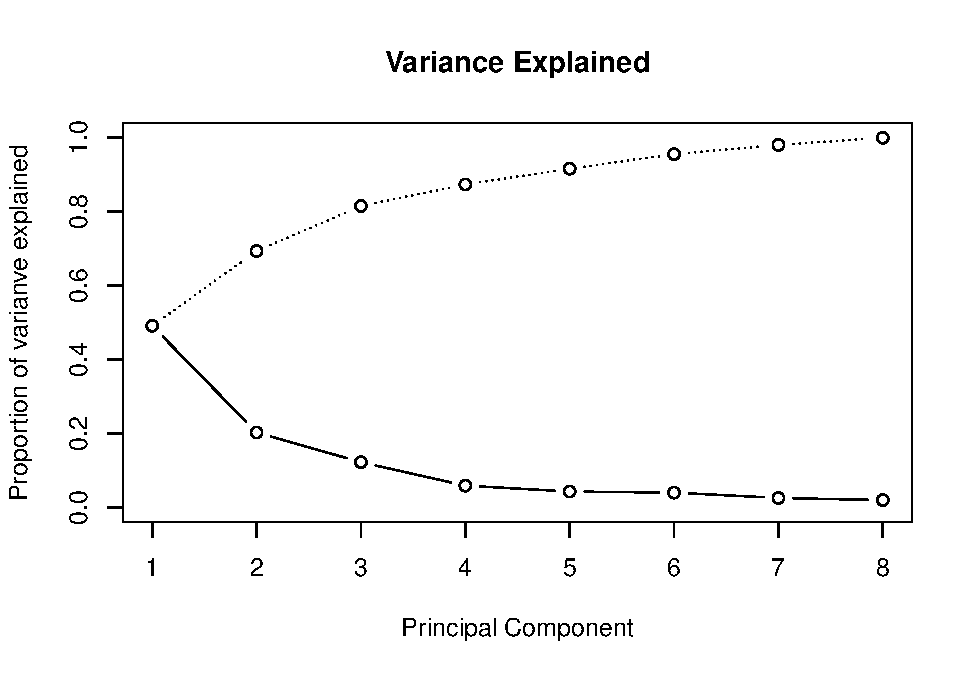
\includegraphics{assignment1_PCA_files/figure-latex/unnamed-chunk-9-1.pdf}

\section{5. Interpretation}

\begin{Shaded}
\begin{Highlighting}[]
\CommentTok{# Eigenvectors}
\NormalTok{evec <-}\StringTok{ }\NormalTok{pr.out}\OperatorTok{$}\NormalTok{rotation}

\CommentTok{# Correlation coefficients between PC's and initial variables}
\NormalTok{varnames <-}\StringTok{ }\KeywordTok{names}\NormalTok{(drugdata)}
\NormalTok{corrcoef <-}\StringTok{ }\KeywordTok{matrix}\NormalTok{(}\DataTypeTok{nrow =} \DecValTok{2}\NormalTok{, }\DataTypeTok{ncol =} \KeywordTok{ncol}\NormalTok{(drugdata), }\DataTypeTok{byrow =}\NormalTok{ T)}
\KeywordTok{colnames}\NormalTok{(corrcoef) <-}\StringTok{ }\NormalTok{varnames}
\KeywordTok{rownames}\NormalTok{(corrcoef) <-}\StringTok{ }\KeywordTok{c}\NormalTok{(}\StringTok{"PC1"}\NormalTok{, }\StringTok{"PC2"}\NormalTok{)}

\ControlFlowTok{for}\NormalTok{( n }\ControlFlowTok{in} \DecValTok{1}\OperatorTok{:}\KeywordTok{length}\NormalTok{(}\KeywordTok{rownames}\NormalTok{(corrcoef)) )\{}
  \ControlFlowTok{for}\NormalTok{( m }\ControlFlowTok{in} \DecValTok{1}\OperatorTok{:}\KeywordTok{nrow}\NormalTok{(evec) )\{}
\NormalTok{    corrcoef[n,m] <-}\StringTok{ }\NormalTok{evec[m,n] }\OperatorTok{*}\StringTok{ }\KeywordTok{sqrt}\NormalTok{(eval)[n]}
\NormalTok{  \}}
\NormalTok{\}}
\NormalTok{corrcoef}
\end{Highlighting}
\end{Shaded}

\begin{verbatim}
##           L500      L1000      L2000      L4000       R500      R1000
## PC1 -0.1654987 -0.2163314 -0.4405707 -1.3442860 -0.1312078 -0.1765976
## PC2 -0.3735063 -0.5066182 -0.7096059  0.1478986 -0.3535584 -0.3967631
##          R2000      R4000
## PC1 -0.3383047 -1.3002910
## PC2 -0.4763866  0.4328621
\end{verbatim}

\begin{Shaded}
\begin{Highlighting}[]
\CommentTok{# First principal component is significantly negatively correlated}
\CommentTok{# with all variables}
\CommentTok{# Second component discriminates between L2000, L4000, R2000, R4000 on one hand}
\CommentTok{# (high dose) and L500, L1000, R500 and R1000 on the other hand (low dose)}
\end{Highlighting}
\end{Shaded}

\begin{Shaded}
\begin{Highlighting}[]
\KeywordTok{biplot}\NormalTok{(pr.out)}
\end{Highlighting}
\end{Shaded}

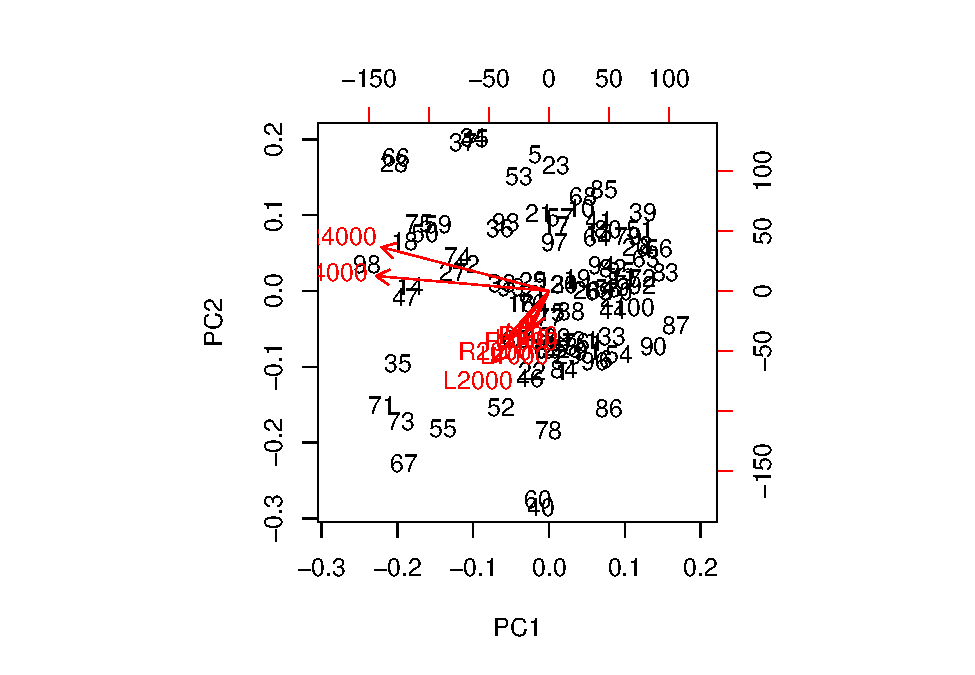
\includegraphics{assignment1_PCA_files/figure-latex/unnamed-chunk-11-1.pdf}

\begin{Shaded}
\begin{Highlighting}[]
\KeywordTok{biplot}\NormalTok{(pr.out, }\DataTypeTok{choices =} \KeywordTok{c}\NormalTok{(}\DecValTok{3}\NormalTok{,}\DecValTok{4}\NormalTok{))}
\end{Highlighting}
\end{Shaded}

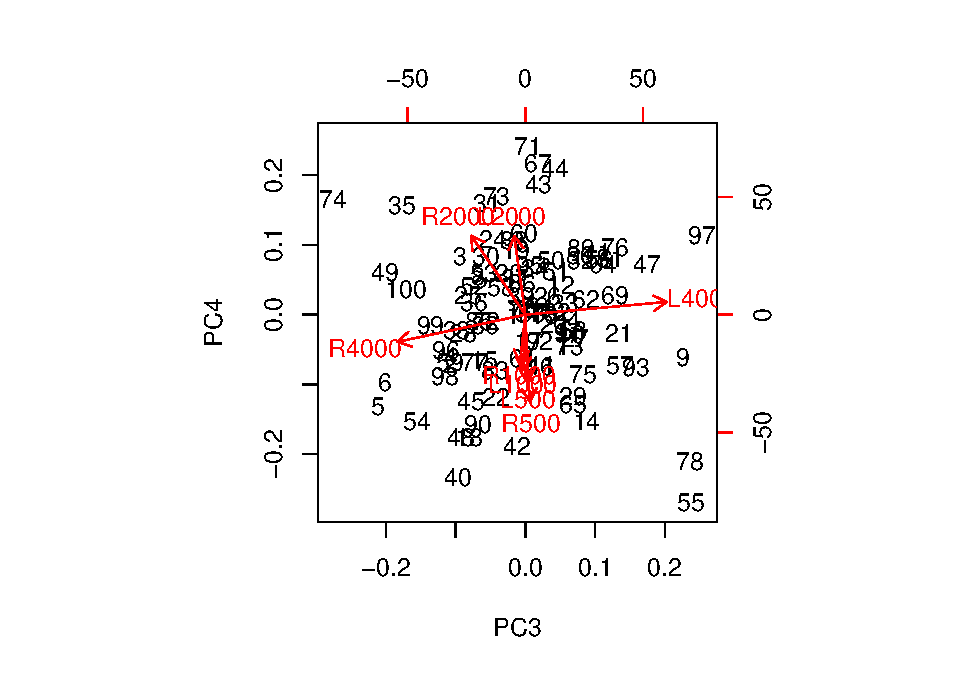
\includegraphics{assignment1_PCA_files/figure-latex/unnamed-chunk-11-2.pdf}

first plot shows two groupings of dosage amount independant of the drug

second plot barely shows any relevant information as there is barely any
group seperation -\textgreater{} was to be expected since they explain
small portion of the variance only

For the majority of the patients, both drugs had barely any effect on
the percentage drop. Lower dose seems to be more effective compared to
higher dose, as with a lower dose more patients had a percentage drop.


\end{document}
